\section{Compressive Failure}

\subsection{Crushing}

You will be familiar with tensile failure from IA, that when the elastic energy released by growing a crack exceeds any work done in creating new surfaces or deforming material at the crack tip then catastrophic failure will occur. This is also intuitively reasonable since the stresses are acting to pull the atoms apart.

In contrast, it is not necessarily clear how a material will fail when the stresses act to push the atoms together. To understand why failure occurs we must consider the stress state more thoroughly.

\FloatBarrier
\begin{figure}[h!]
\centering
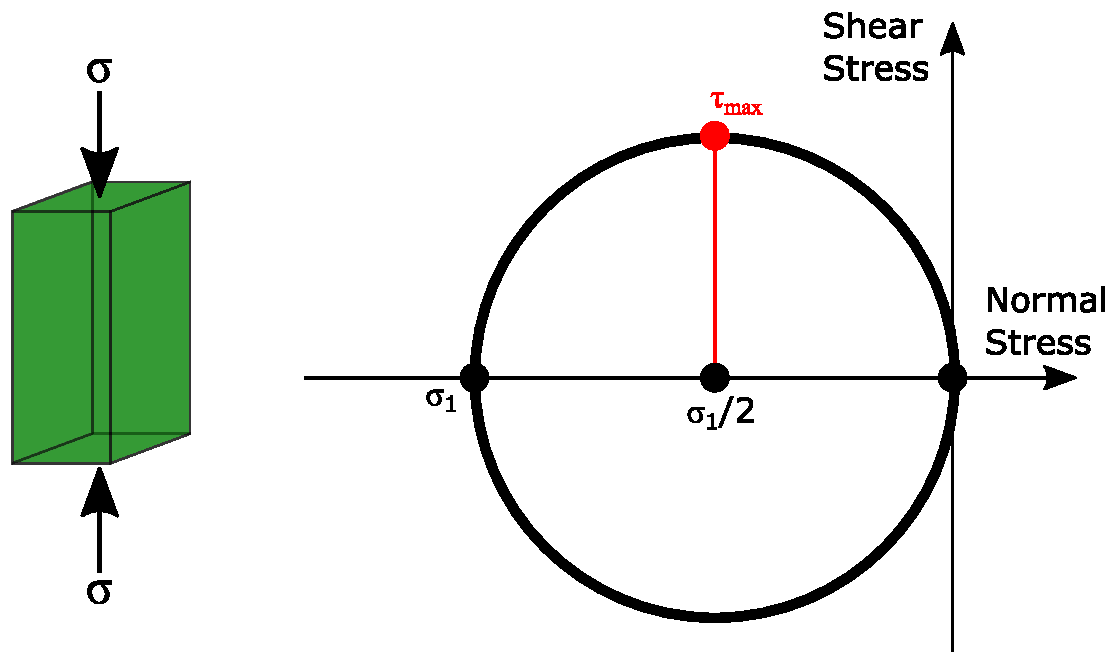
\includegraphics[width=0.6\textwidth]{compression_and_stress_state}
\caption{The stress state in a uniaxial compression test.\label{fig:compressive_stress_state}}
\end{figure}

\FloatBarrier

The Mohr's circle shown in \autoref{fig:compressive_stress_state} shows that there will be a shear stress in the material, that has a maximum value on planes inclined by \SI{45}{\degree} to the compression axis. There will be a driving force for crack growth along these planes:

\FloatBarrier
\begin{figure}
\centering
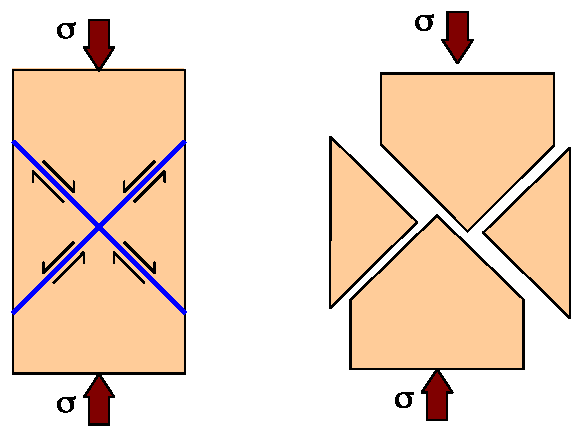
\includegraphics[width=0.7\textwidth]{crushing_schematic}
\caption{Schematic showing the way that shear stresses can give rise to a driving force for crack growth.}
\end{figure}

\FloatBarrier

\FloatBarrier
\begin{figure}[h!]
\centering
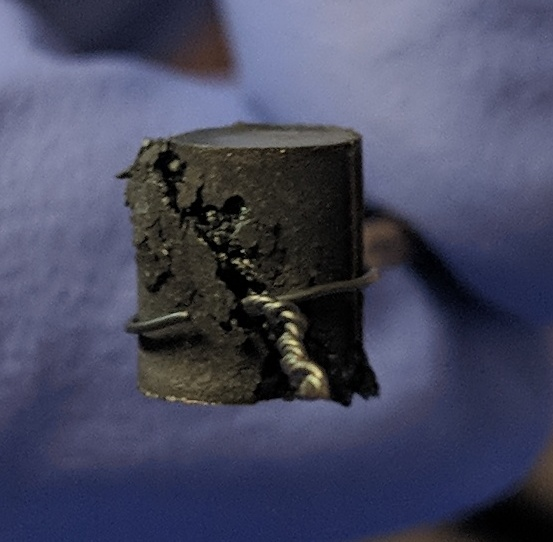
\includegraphics[width=0.5\textwidth]{crushed}
\caption{The failure of a nickel based superalloy compressed at \SI{1000}{\celsius}. The wire around the cylinder is a thermocouple to measure the temperature. With thanks to (soon to be Dr) Amy Goodfellow for the photograph.\label{fig:crushed}}
\end{figure}

\FloatBarrier



This is indeed seen in real materials, as shown in \autoref{fig:crushed}. Note that the crack seems to be intergranular, and runs across the sample at roughly \SI{45}{\degree}. The idealised case would have more than one single plane of failure, as shown in the schematic, but misalignment of the compression axis can add additional shear components to the stress state that favour one particular plane.

\subsection{Buckling}
\subsubsection{Elastic buckling}


Crushing of the material is only one of the ways that compressive failure may occur. If instead the elastic deformation of the material is large then this can lead to failure at loads lower than the crushing strength.

We will start by considering the compression of a freely hinged beam, i.e. the ends are on freely rotating pins, and the upper pin remains aligned vertically above the other:

\FloatBarrier
\begin{figure}[h!]
\centering
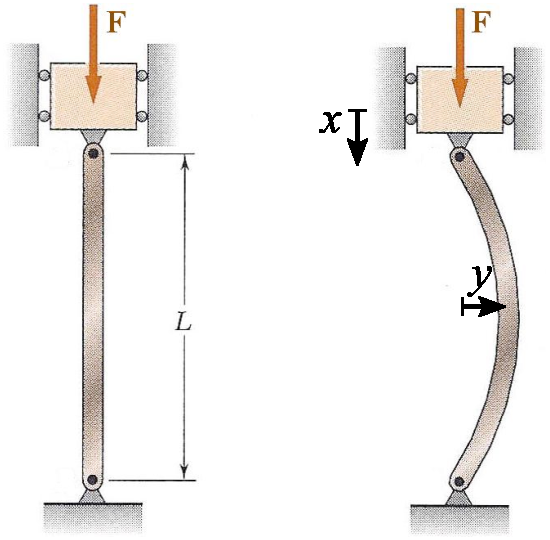
\includegraphics[width=0.6\textwidth]{freely_hinged_beam}
\caption{Compressive loading of a freely hinged beam that deflects elastically.\label{fig:free_hinge_deflection}}
\end{figure}
\FloatBarrier


In order to make this problem tractable we must assume a number of things:
\begin{enumerate}
\item The cross section is uniform. \begin{annotation} i.e.\ the beam doesn't taper. \end{annotation}
\item The material is homogeneous, isotropic and linear elastic.
\item The self weight (the forces due to the weight of the beam itself are negligible compared to the applied load.
\item The force is axial -- there is no eccentricity. \begin{annotation}  This is actually v.\ difficult to do in practice.\end{annotation}
\end{enumerate}

So considering the scenario shown in \autoref{fig:free_hinge_deflection}, there are two energy changes, firstly the work done by the applied force if the ends of the beam move:
\begin{equation}
\delta U_{\text{F}} = -F x \qquad\begin{annotation}
\text{-ve since the gpe of the system decreases.}
\end{annotation}
\end{equation}
\begin{annotation}
This energy change will favour buckling of the beam.
\end{annotation}

However the deflection of the beam will cause an internal energy change:
\begin{equation}
\begin{annotation}
\delta U_{\text{E}} > 0 \qquad \text{Energy is raised so opposes buckling.}
\end{annotation}
\end{equation}

This leads to a simple criterion as to whether buckling occurs or not:

\begin{equation}
\text{For buckling:} \qquad |\delta U_{\text{F}}| > |\delta U_{\text{E}}|
\end{equation}

If this is true the overall energy change will be negative and therefore favourable. To determine this we must consider the elastic energy of the beam, as a function of the displacement $y$.


If we consider a point along the beam, denoted $Q$, while the force applied is exactly equal to the critical load and the beam is in static equilibrium:
\FloatBarrier
\begin{figure}[h!]
\centering
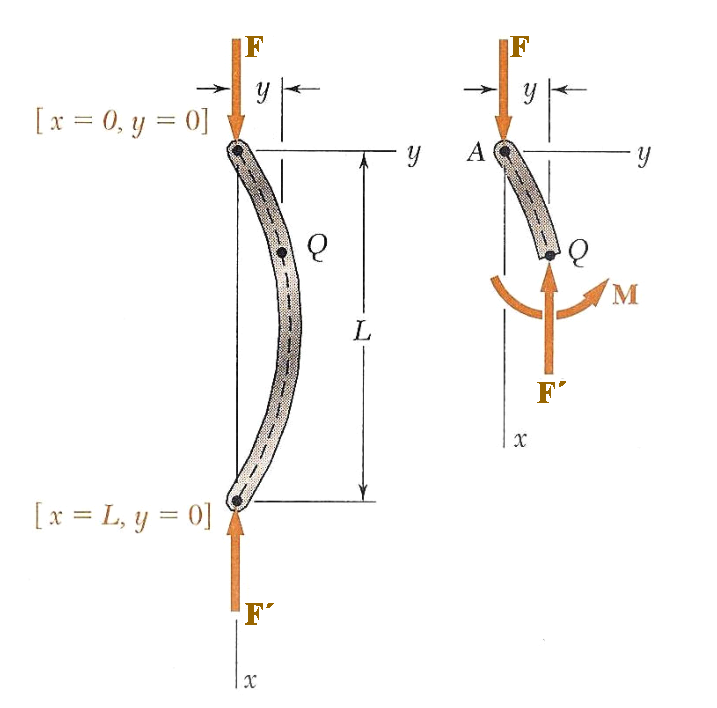
\includegraphics[width=0.5\textwidth]{moments_in_buckling}
\caption{}
\end{figure}
\FloatBarrier
We can say that the moment due to the external forces at the point $Q$ is:
\begin{equation}
M=-Fy
\end{equation}
which must be balanced by the internal moments generated by the stresses in the material. We can use the beam bending equation from earlier:
\begin{equation}
M=\kappa E I = \frac{d^2y}{dx^2}EI
\end{equation}

\begin{annotation}
Defining $ x$ and $y$ in this odd way ensures that these differential equations look the same.
\end{annotation}

These moments can be  set equal to each other:
\begin{equation}
-Fy = \frac{d^2y}{dx^2}EI \label{eqn:diff_equation}
\end{equation}
\begin{annotation}
\begin{equation}
\frac{d^2y}{dx^2} + \frac{Fy}{EI} = 0
\end{equation}
\end{annotation}

This is similar to the equation for beam bending, \autoref{eqn:beam_curvature}, but here the moment is also a function of the displacement, $y$, and the moment will increase as the deflection increases.

\autoref{eqn:diff_equation} is of the form:
\begin{equation}
\frac{d^2y}{dx^2} + k^2y = 0
\end{equation}
where $k=\frac{F}{EI}$, which is an ordinary second order differential equation and has a general solution of the form:
\begin{equation}
y = A\sin kx + B \cos kx
\end{equation}


The boundary conditions are that the ends of the beam remain aligned vertically, so that:

\begin{equation}
x=0, x=L \implies y = 0
\end{equation}

Using $y=0$ when $x=0$:
\begin{equation}
A \sin 0 + B \cos 0 = 0
\end{equation}
which implies that $B=0$. \begin{annotation} This leaves the form as a simple sine curve, $y=A\sin kx$ \end{annotation}
\\

Then using $y=0$ when $x=L$:
\begin{equation}
A \sin kL = 0
\end{equation}
One simple solution to this is that $A=0$, however this is simply the case when the beam has not deflected at all and therefore can be discounted. If $A \neq 0$ then:
\begin{align}
\sin kL = 0 \\
\implies kL = n\pi \qquad \text{where} \,\, n \,\, \text{is an integer.}\nonumber
\end{align}

Recalling that $k^2 = F/EI$ we can write that:
\begin{equation}
\frac{F_{\text{EB}}}{EI} = \frac{n^2\pi^2}{L^2}
\end{equation}
and therefore finally the force required for elastic buckling is given by:
\begin{equation}
F_{\text{EB}} = \frac{n^2 \pi^2 EI}{L^2}
\end{equation}

This gives rise to the possibility of more than one configuration of buckling since $n$ can take any integer value, as shown in \autoref{fig:buckling_configs}. However, since the force required for each mode increases with $|n|$ the beam will fail by buckling with $n=\pm1$, and $|n|>1$ will not occur unless further constraints are placed on the beam.

\begin{figure}
\centering
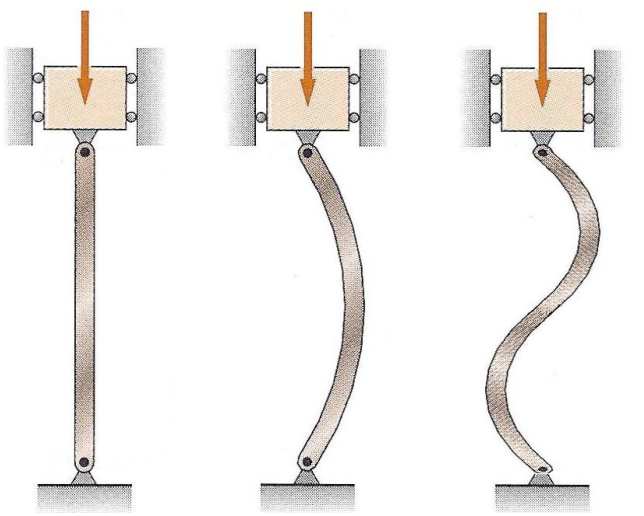
\includegraphics[]{buckling_configs}
\caption{Possible configurations of the elastic buckling of a beam. Those with $n > 1$ are of no practical interest.\label{fig:buckling_configs}}
\end{figure}

For forces lower than this any perturbation sideways will raise the energy of the system and the beam will straighten itself to lower the elastic energy, and hence will not buckle. When $F=F_{\text{EB}}$ static equilibrium in the $n=\pm1$ configuration is achieved, and if the force exceeds this then the column becomes unstable and the beam will fail catastrophically as soon as it is perturbed from perfectly straight


The failure stress of a column, by elastic buckling is therefore:
\begin{equation}
F_{\text{EB}} = \frac{\pi^2 EI}{L^2}
\end{equation}

This represents an upper bound on the failure load of a beam, since defects in the material such as inhomogeneity or pores/dimensional variations could cause the true value to be lower. It's also unlikely that the loading will be purely axial and this would also lower the failure load.

\subsubsection{The effects of end constraints}

Many real scenarios will not have freely rotating ends but instead will have fixed or clamped ends. First let's consider the case of one end clamped and one end free to rotate:
\FloatBarrier
\begin{figure}[h!]
\centering
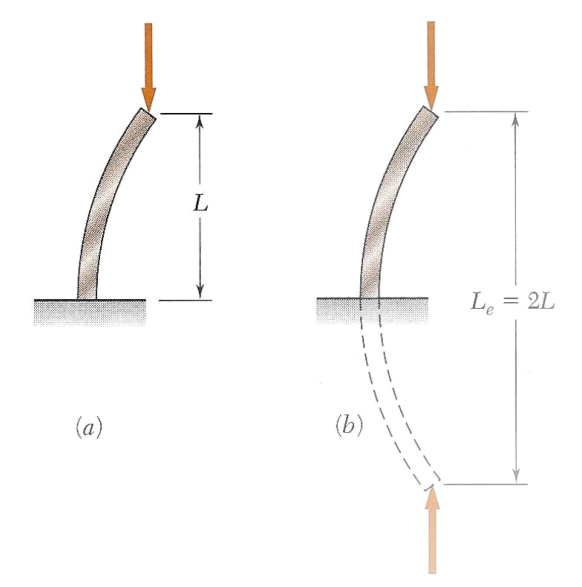
\includegraphics[width=0.5\textwidth]{one_fixed_one_free}
\caption{The buckling load of a beam with one fixed end can be easily calculated by considering an ``effective length''.   }

\begin{annotation}
The length $2L$ is equivalent to the $L$ used in the derivation for two free ends. 
\end{annotation}
\end{figure}
\FloatBarrier

By using the ``effective length'' the elastic buckling force is:
\begin{equation}
F_{\text{EB}} = \frac{\pi^2EI}{(2L)^2} = \frac{1}{4}\frac{\pi^2EI}{L^2}
\end{equation}
\begin{annotation}
The failure load has been reduced by a factor of 4.
\end{annotation}

The other likely scenario is when both ends are fixed, and a similar approach is possible:
\FloatBarrier
\begin{figure}[h!]
\centering
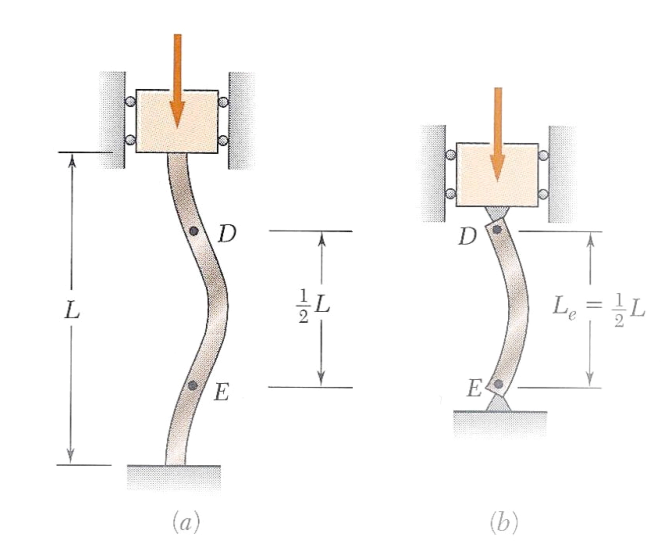
\includegraphics[]{two_fixed_ends}
\caption{The radius of curvature has decreased, and the new shape has an effective length of $L/2$.}
\end{figure}
\FloatBarrier

This alters the force required for elastic buckling to be:
\begin{equation}
\begin{annotation}
F_{\text{EB}} = \frac{\pi^2EI}{(L/2)^2} = 4 \frac{\pi^2EI}{L^2}
\end{annotation}
\end{equation}

\begin{quotation}
The buckling load has increased by a factor of 4.
\end{quotation}


We can write a final expression where the nature of the ends of the beam are included as a constant:
\begin{equation}
F_{\text{EB}} = c \frac{\pi^2 EI}{L^2}
\end{equation}
where $c$ may take a value of $^1\!/_4$, $1$ or $4$ depending on the situation in question.


\subsubsection{The effect of aspect ratio}

We can write an expression for the stress in a beam when elastic buckling occurs:
\begin{equation}
\sigma_{\text{EB}} = \frac{F_{\text{EB}}}{A} = c \frac{\pi^2 E I }{L^2 A}
\end{equation}
and assuming that we have a cylindrical beam we can link $I$ and $A$ to the radius, $R$:
\begin{equation}
\begin{annotation}
I = \frac{\pi R^4}{4} \qquad \qquad A= \pi R^2
\end{annotation}
\end{equation}
and substituting these in:
\begin{equation}
\sigma_{\text{EB}} = \frac{c}{4} \frac{\pi^2 E}{(L/R)^2}
\end{equation}

Thus the stress at which a beam will buckle depends on the aspect ratio. This is perhaps familiar from every day life, that as a beam becomes longer and more slender the stress required for it to fail by elastic buckling decreases.

The ratio $L/R$ is called the slenderness ratio and is the crucial geometric factor in the failure of a beam. The only material property that affects the the buckling stress of a beam is the Young's modulus $E$. These two effects can be represented graphically:

\FloatBarrier
\begin{figure}[h!]
\centering
\begingroup%
  \makeatletter%
  \providecommand\color[2][]{%
    \errmessage{(Inkscape) Color is used for the text in Inkscape, but the package 'color.sty' is not loaded}%
    \renewcommand\color[2][]{}%
  }%
  \providecommand\transparent[1]{%
    \errmessage{(Inkscape) Transparency is used (non-zero) for the text in Inkscape, but the package 'transparent.sty' is not loaded}%
    \renewcommand\transparent[1]{}%
  }%
  \providecommand\rotatebox[2]{#2}%
  \ifx\svgwidth\undefined%
    \setlength{\unitlength}{397.00601893bp}%
    \ifx\svgscale\undefined%
      \relax%
    \else%
      \setlength{\unitlength}{\unitlength * \real{\svgscale}}%
    \fi%
  \else%
    \setlength{\unitlength}{\svgwidth}%
  \fi%
  \global\let\svgwidth\undefined%
  \global\let\svgscale\undefined%
  \makeatother%
  \begin{picture}(1,0.55617582)%
  \begin{annotation}
    \put(0,0){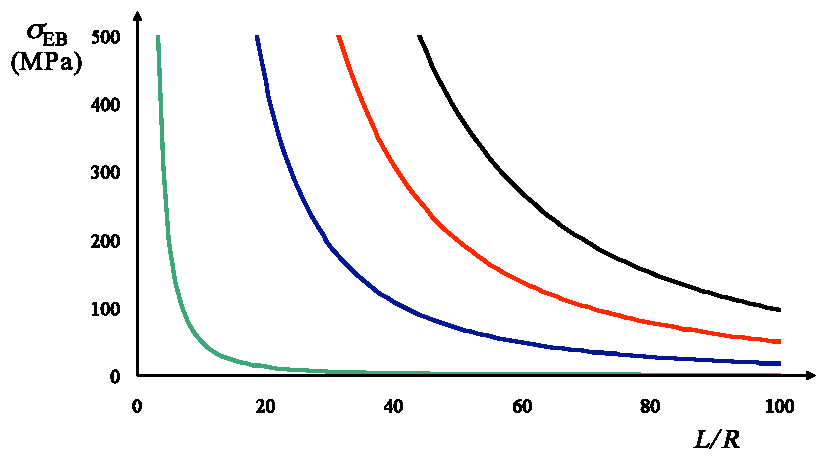
\includegraphics[width=\unitlength,page=1]{slenderness_buckling.pdf}}%
    \put(0.32520198,0.52828452){\makebox(0,0)[lb]{\smash{For \textit{c}=1}}}%
    \put(0.34476807,0.1194207){\makebox(0,0)[lb]{\smash{Nylon}}}%
    \put(0.55678051,0.16588762){\makebox(0,0)[lb]{\smash{Al}}}%
    \put(0.68741711,0.19937701){\makebox(0,0)[lb]{\smash{Fe}}}%
    \put(0.79951108,0.23074506){\makebox(0,0)[lb]{\smash{\ce{Al2O3}}}}%
    \put(0,0){\includegraphics[width=\unitlength,page=2]{slenderness_buckling.pdf}}%
    \put(0.7158491,0.52){\makebox(0,0)[lb]{\smash{Increasing Stiffness}}}%
    \put(0.7158491,0.48){\makebox(0,0)[lb]{\smash{Buckling is less likely}}}%
    \put(0.7158491,0.44){\makebox(0,0)[lb]{\smash{Survive higher stress}}}%
    \put(0.7158491,0.40){\makebox(0,0)[lb]{\smash{Or higher slenderness}}}%
    \end{annotation}
  \end{picture}%
\endgroup%
\caption{The variation of the buckling stress with slenderness ratio for a number of different material stiffnesses}
\end{figure}
\FloatBarrier

\subsubsection{The effect of cross-section shape}

As we know from IA and have recapped earlier in the course, the shape of a beam's cross-section is important when considering the deflection of the beam, this is quantified by the second moment of area, $I$. In a horizontal beam we already know which way the moment will be applied and this leads to the I-beam we are familiar with. However in buckling the beam might deflect in any direction and so is most likely to deflect such that $EI$, the beam stiffness, is smallest, and since $E$ usually doesn't vary this means the direction for which $I$ is smallest.

\FloatBarrier

\begin{figure}[h!t]
\centering
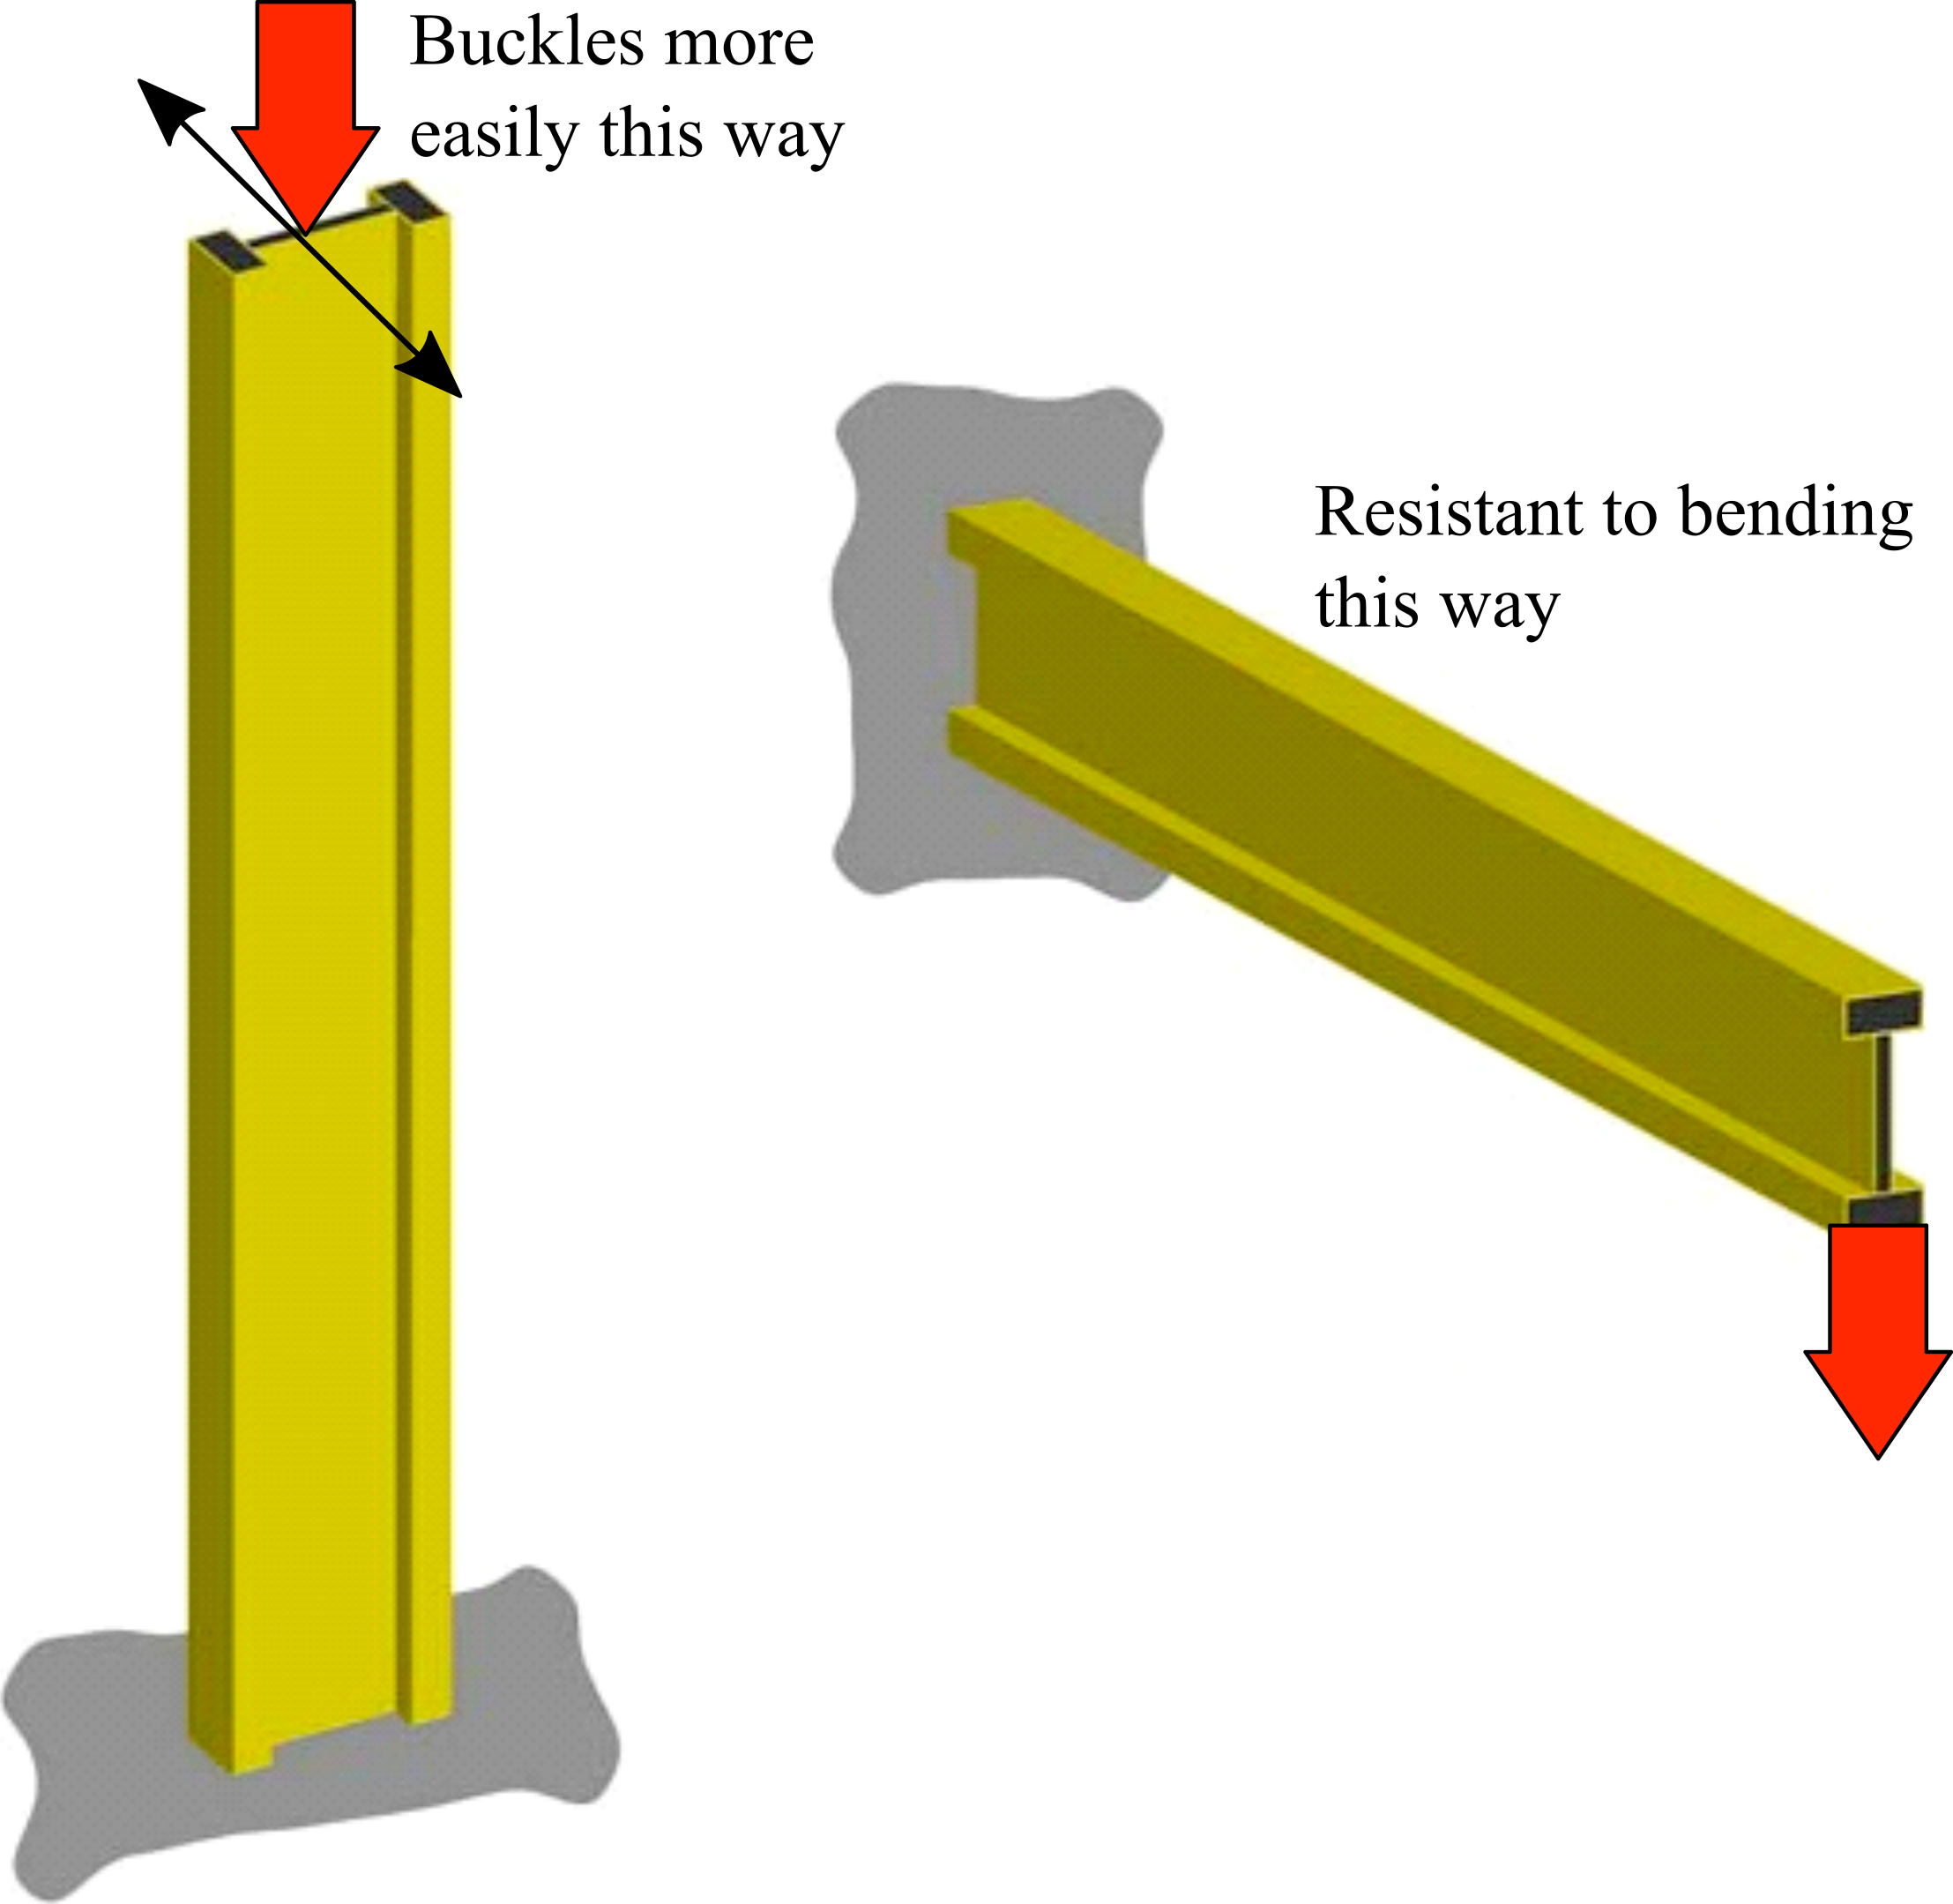
\includegraphics[width=9cm]{I_beam}
\end{figure}
\FloatBarrier


For this reason there is little benefit to shapes such as I-beams, and instead a cylindrical cross sections, or other rotationally symmetric shapes (squares, equilateral triangles etc.), are best (for a given column height and a given volume of material).

This leads to a way in which the volume (and therefore the cost) of material can be kept constant, while increasing the second moment of area. A hollow cross section will result in moving material away from the neutral axis and so increase $I$, and increase the resistance to buckling.

\FloatBarrier
\begin{figure}[h!b]
    \centering
    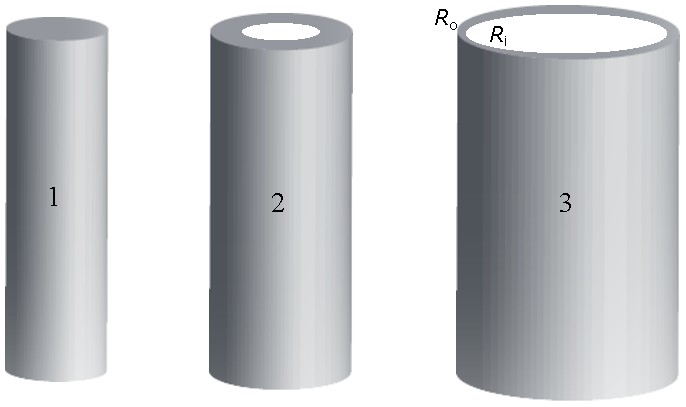
\includegraphics[width=0.6\textwidth]{hollow_cylinders}
    \caption{Increasing the second moment of area by using a hollow cylinder (for a given volume of material). The greater the radius, the greater the resistance to elastic buckling.\label{fig:my_label}}
\end{figure}

The second moment of area for a hollow cylinder is given by:

\begin{equation}
    \begin{annotation}
    I = \frac{\pi (R_{\text{o}}^4 - R_{\text{i}}^4)}{4}
    \end{annotation}
\end{equation}
\begin{annotation}
Therefore $I_3 > I_2 > I_1$
\end{annotation}

Hence the use of hollow cylinders to mount road signs or build scaffolding.

\subsubsection{Does elastic buckling cause failure?}

Elastic buckling thus far has been described in purely elastic, and therefore reversible and recoverable, terms. However the change in shape usually leads to other forms of failure, such as brittle fracture in the regions of material under tensile stress, plastic deformation in either tension or compression, or local buckling may occur (we will discuss this shortly).

Reaching failure or not often depends on the loading scenario. Consider a test performed under {\bf displacement control}, in which we apply sufficient force to the end plates of a column to control the distance between them. Initially there will be simple elastic deformation of the material, but soon the buckling force is reached. However, the buckling will not lead to catastrophic collapse because as the force resisting the motion of the end plates drops, so too does the applied force. Instead the buckling will advance in a stable manner and can be reversed unless some other material failure has occurred.

\begin{annotation}
The load is not free to lower the energy of the system after $F_{\text{EB}}$ has been reached, instead the applied force is reduced to maintain a fixed displacement.
\end{annotation}

Alternatively a column may be tested under {\bf load control}. This is achieved by gradually increasing the load and measuring the displacement that arises (the simplest form of load control would be to stack weights on top of a column). Recalling the buckling will occur when the energy changes driving it exceeds the energy changes resisting it. This means that buckling will be sudden and the ends of the column will come together. If the material can recover from large strains, e.g.\ a rubber, then the column may recover when the load is reduced, but otheriwse will likely have failed due to large stresses and strains that develop in the beam.

\begin{annotation}
The load is free to continue doing work and lower the energy of the system, leading to complete failure.
\end{annotation}

\subsection{Local Buckling}

If we assume that elastic buckling is the only mode of failure that can occur (below an upper bound on the strength which is the ordinary compressive strength of the material) then this leads us to the conclusion that failure of the structure can be avoided simply by increasing the radius of a hollow cylindrical column, without increasing the amount of material.

Howver as the radius of the cross section increases the wall thickness must decrease (assuming a constant volume of material). There is a lower limit to the wall thickness that can be used, and below a critical thickness failure will occur by {\bf local buckling}. A paper straw crumpling is an example of this, and unlike elastic buckling, is always irreversible.

The force required for local buckling is given by:
\begin{equation}
    F_{\text{lb}} = k\pi E t^2
\end{equation}
where $t$ is the wall thickness, $E$ is the Young's modulus and $k \approx 0.5$ is a constant that depends of the surface imperfections. 

A drinks can is a good example of a structure that we know will fail by local buckling. We can calculate the force required for failure:

\begin{annotation}
\begin{figure}[t!]
    \centering
    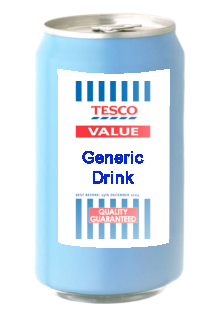
\includegraphics{generic_drink}
\end{figure}
\FloatBarrier

$$
t \approx \SI{100}{\micro\meter} \qquad \text{and Al:} \qquad E \approx \SI{70}{\giga\pascal}
$$

$$ F = 0.5  \pi ( 70\times 10^9 )(100\times 10^{-6})^2\approx \SI{1.1}{\kilo\newton} $$

$$\implies \sigma = \SI{50}{\mega\pascal}$$
\end{annotation}

\subsubsection{The effect of internal pressure}

\FloatBarrier
\begin{figure}[h!]
    \centering
    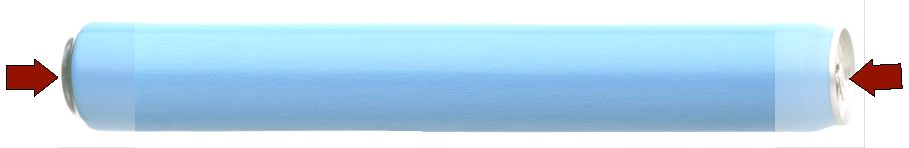
\includegraphics[width=\textwidth]{long_can}
\end{figure}
\FloatBarrier




